In Sec.~\ref{sec:method_gen_fuzzy}, we describe the generation of fuzzy trap sequences from a reference trap sequence $(X_{\text{ref}})$. First, we tokenize the reference trap sequence using the tokenizer of a masked language model MLM, resulting in $T_{\text{MLM}}(X_{\text{ref}}) = \{t_1,\ldots,t_N\}$. Due to the different tokenization of $T_{\text{ref}}$ and $T_{\text{MLM}}$, $N$ differs from $L_{\text{ref}}$. Fig~\ref{fig:tokens_ppl} (a) shows how the $N=|T_{\text{MLM}}(X_{\text{ref}})|$ is distributed for $100$ reference trap sequences - which all have $L_{\text{ref}}=100$. 

Next, to generate fuzzy trap sequences, we replace $R$ tokens by sampling from the top $k$ tokens predicted by the MLM. For smaller values of $k$, we expect more meaningful token replacements to be made than for larger values of $k$. Indeed, when $k$ equals the size of the vocabulary of the MLM, or $k=|\mathcal{V}_{\text{MLM}}|$, we would effectively replace the token with a random other token regardless of its context in the reference trap sequence. This will likely impact the difference across fuzzy duplicates. We quantify this difference with the commonly used notion of \emph{perplexity}. For the sequence of textual characters $X$, tokenized as $T(X) = \{t_1,\ldots,t_L\}$, we denote the loss of language model $\textit{LM}$ with tokenizer $T$ as:

\begin{equation}
\label{eq:loss}
\mathcal{L}_{\textit{LM}}(X) = -\frac{1}{L}\sum_{i=1}^{L} \log\left( \textit{LM}_{\theta}(t_i | t_1 \ldots, t_{i-1})\right) 
\end{equation}

Perplexity is then computed as the exponent of the loss, i.e. $\mathcal{P}_{\textit{LM}}(X) = \exp\left(\mathcal{L}_{\textit{LM}}(X)\right)$. The higher the value of perplexity, the more 'surprised' language model $\textit{LM}$ is to observe sequence $X$. 

We now compute how the perplexity of the fuzzy trap sequences differs from the perplexity of the reference trap sequence. We generate synthetic reference trap sequences of length $L_{\text{ref}}(X_{\text{ref}})=100$ and perplexity $90 \leq \mathcal{P}_{\textit{LM}_{\text{ref}}}(X_{\text{ref}}) < 100$. Making $R$ replacements in such a sequence will have undoubtedly altered this perplexity. Fig~\ref{fig:tokens_ppl} (b) shows how the perplexity of fuzzy trap sequences computed using $\textit{LM}_{\text{ref}}$ varies for increasing number of replacements $R$. We find that, when more tokens are replaced, the perplexity indeed increases compared to the perplexity of the reference trap sequence $X_{\text{ref}}$, and more rapidly so when token replacements are made with higher values of $k$..  

\begin{figure*}[ht]
\centering
\subfigure{
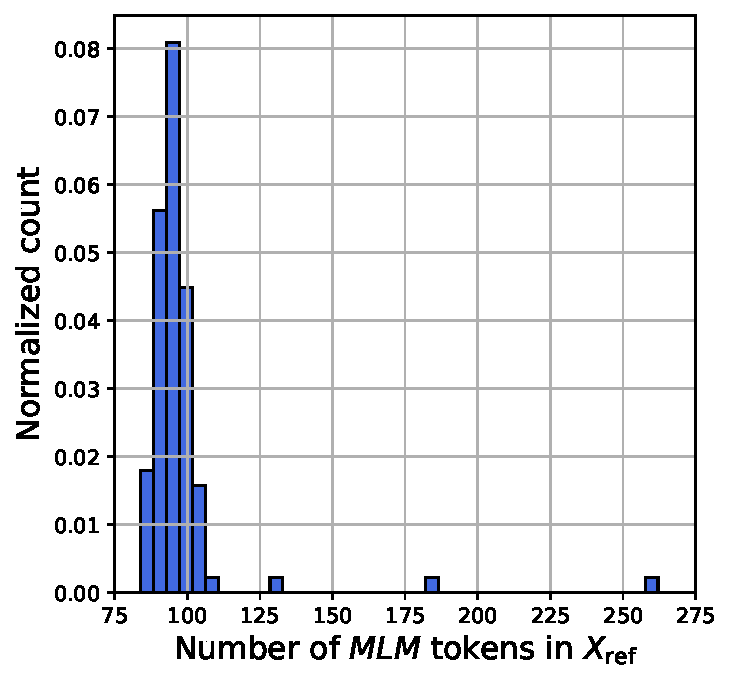
\includegraphics[width=0.35\linewidth]{figures/MLM_tokens.pdf}
}
\subfigure{
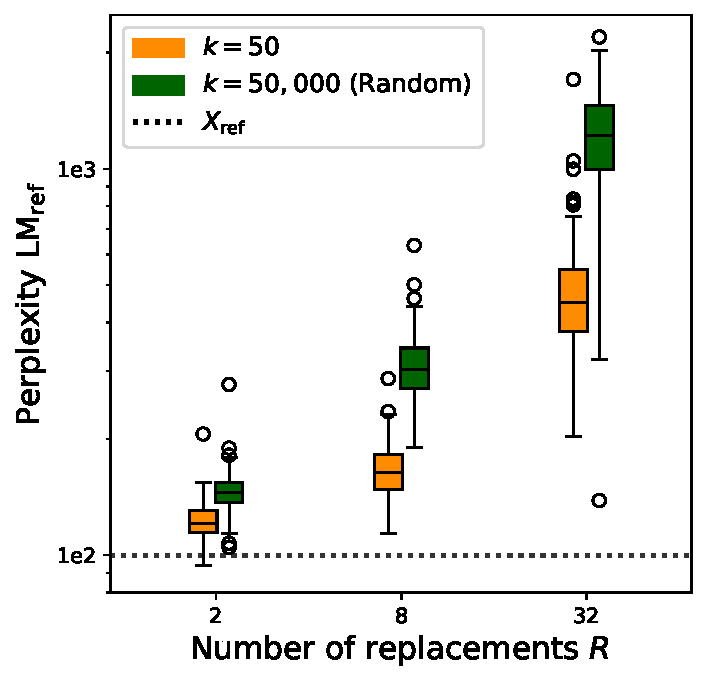
\includegraphics[width=0.35\linewidth]{figures/llama_ppl_neardupls.pdf}
}
\caption{\textbf{Characterizing fuzzy trap sequences.} (a) The distribution of number of tokens $|T_{\text{MLM}}(X_{\text{ref}})|$ of $100$ reference trap sequences. (b) The perplexity computed using $\textit{LM}_{\text{ref}}$ each for $100$ fuzzy trap sequences for token replacement strategies for different values of $k$ across values for $R$.} 
\label{fig:tokens_ppl}
\end{figure*}